%!TEX root = ../rules-working.tex
%LTeX: enabled=false

\begin{twocolumnfigure}[tp]
\addedin{3A}{3A-ship-movement}{

\begin{fitheight}{4.4\standardhexwidth}

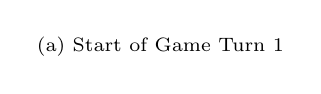
\begin{tikzpicture}
    \setfiguresize{-2.4}{-1.6}{+1.6}{+2.8}
    \drawhexgrid{-2}{-1}{4}{3}
    \drawshipcounter{0.0}{-0.0}{90}{}{}
    \miniathex{-0.5}{+2.20}{\node [anchor=south] {\scriptsize (a) Start of Game Turn 1};}
\end{tikzpicture}

\hspace{5mm}

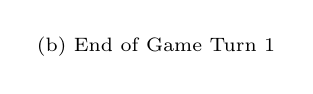
\begin{tikzpicture}
    \setfiguresize{-2.4}{-1.6}{+1.6}{+2.8}
    \drawhexgrid{-2}{-1}{4}{3}
    \drawshipcounter{0.0}{-0.0}{90}{}{}
    \miniathex{-0.5}{+2.20}{\node [anchor=south] {\scriptsize (b) End of Game Turn 1};}
\end{tikzpicture}

\hspace{5mm}

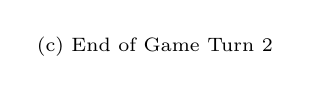
\begin{tikzpicture}
    \setfiguresize{-2.4}{-1.6}{+1.6}{+2.8}
    \drawhexgrid{-2}{-1}{4}{3}
    \drawshipcounter{0.0}{-0.0}{150}{}{}
    \miniathex{-0.5}{+2.20}{\node [anchor=south] {\scriptsize (c) End of Game Turn 2};}
\end{tikzpicture}

\hspace{5mm}

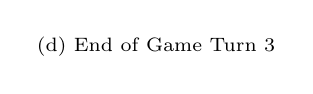
\begin{tikzpicture}
    \setfiguresize{-2.4}{-1.6}{+1.6}{+2.8}
    \drawhexgrid{-2}{-1}{4}{3}
    \drawshipcounter{0.0}{-0.0}{150}{}{}
    \miniathex{-0.5}{+2.20}{\node [anchor=south] {\scriptsize (d) End of Game Turn 3};}
\end{tikzpicture}

\hspace{5mm}

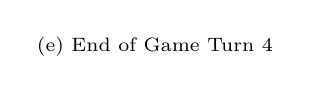
\begin{tikzpicture}
    \setfiguresize{-2.4}{-1.6}{+1.6}{+2.8}
    \drawhexgrid{-2}{-1}{4}{3}
    \drawshipcounter{-1.0}{0.5}{210}{}{}
    \miniathex{-0.5}{+2.20}{\node [anchor=south] {\scriptsize (e) End of Game Turn 4};}
\end{tikzpicture}

\end{fitheight}

\figurecaption{figure:ship-movement-example}{The position of HMS {\itshape Arrow} during the ship movement example in the text.}

}
\end{twocolumnfigure}